\documentclass[11pt,a4paper]{article}

% ---------------------------------------------------------------
% 컴파일: xelatex KAMP_report.tex (2회)  또는  latexmk -xelatex KAMP_report.tex
% ---------------------------------------------------------------
\usepackage[hangul]{kotex}
\setmainhangulfont{Malgun Gothic}
\setsanshangulfont{Malgun Gothic}
\setmainfont{Malgun Gothic}

\usepackage[margin=2.2cm]{geometry}
\usepackage{graphicx}
\usepackage{booktabs}
\usepackage{array}
\usepackage{float}
\usepackage[font=small,labelfont=bf]{caption}
\usepackage{enumitem}
\usepackage{xcolor}
\usepackage[most]{tcolorbox}
\usepackage{amsmath}
\usepackage[hidelinks]{hyperref}

\definecolor{accent}{HTML}{2A78D6}
\definecolor{warn}{HTML}{EB6834}
\setlist{itemsep=2pt,topsep=4pt}
\linespread{1.25}
\graphicspath{{figures/}}

\newtcolorbox{keybox}[1]{colback=accent!5,colframe=accent,boxrule=0.6pt,arc=2pt,
  left=6pt,right=6pt,top=4pt,bottom=4pt,title={#1},fonttitle=\bfseries,coltitle=white}
\newtcolorbox{warnbox}[1]{colback=warn!6,colframe=warn,boxrule=0.6pt,arc=2pt,
  left=6pt,right=6pt,top=4pt,bottom=4pt,title={#1},fonttitle=\bfseries,coltitle=white}

\newcommand{\code}[1]{\texttt{\small #1}}

\title{\textbf{제조 생산데이터 기반 전력사용량 예측 및\\최대피크 위험조건 분석}\\[4pt]
\large KAMP 자원 최적화 AI 데이터셋 --- 과제 ⑤ 분석 보고서}
\author{}
\date{2026년 10월}

\begin{document}
\maketitle
\thispagestyle{empty}

\begin{keybox}{요약}
\begin{itemize}[leftmargin=12pt]
  \item 2021년 1월 1일 $\sim$ 9월 14일 15분 단위 전력·생산 데이터(24,672행)로 XGBoost 기반 전력사용량 예측 모델을 개발하였다.
  \item 초기 모델(Feature4)은 15분 앞 예측에서 Test $R^2=0.983$을 보였으나, 직전 값을 그대로 쓰는 Persistence($R^2=0.953$) 대비 개선은 $+0.03$이었고, 시간 단위 생산실적의 선(先)사용, 피크 과소예측, 평일 휴무 미반영이라는 한계를 확인하였다.
  \item 개선 모델은 예측 구간(15분·1시간·24시간)과 정보 가용성(실적기반·계획기반)을 분리하여 평가하였다. \textbf{24시간 앞 예측에서 Persistence $R^2=0.10$ 대비 실적기반 0.85, 계획기반 0.90}을 달성하였다.
  \item 검증 구간에서 경보 임계값을 선택하여 15분 앞 고전력 경보의 Recall을 0.60에서 0.82로 높였다.
  \item 월별 최대피크 9건은 모두 \textbf{08:30$\sim$11:30, 생산지속 상태}에서 발생했으며, 피크 직전 1시간 동안 평균 전력이 134에서 212로 급상승하였다. 이를 근거로 아침 설비 순차 가동과 오전 고부하 생산의 시간대 이동을 저감방안으로 제안한다.
\end{itemize}
\end{keybox}

\tableofcontents
\newpage

% ===============================================================
\section{과제 개요}
% ===============================================================
제조기업의 전력사용량은 설비 동시 가동, 생산량 변화, 제품 전환, 교대시간 및 계절 요인에 따라 크게 변한다. 최대수요전력이 예상보다 높아지면 전력비용이 증가하고, 특정 시간대에 부하가 집중되면 생산 운영의 안정성도 낮아진다. 과제는 다음 세 가지를 요구한다.

\begin{enumerate}[label=\textbf{\arabic*)}]
  \item 향후 지정된 시간구간의 전력사용량을 예측하는 AI 모델 개발
  \item 예측오차가 크게 발생하는 생산조건과 최대전력 피크 발생 조건 분석
  \item 생산일정 또는 설비가동 시점 조정을 통한 피크전력 저감방안 제안
\end{enumerate}

본 보고서는 초기 모델(제2--4장)을 설계하고 그 한계를 진단한 뒤, 이를 보완한 개선 모델(제5--6장)을 제시한다. 이어 오차·피크 조건을 분석하고(제7장) 저감방안을 제안한다(제8장).

% ===============================================================
\section{데이터}
% ===============================================================
\subsection{데이터 구성}
주 데이터 \code{Power15MinClean\_NoDatetime.csv}는 2021-01-01 00:15부터 2021-09-15 00:00까지 15분 간격 24,672행(257일 $\times$ 96칸, 결측 시점 없음), 17개 열로 구성된다.

\begin{table}[H]
\centering\small
\begin{tabular}{>{\raggedright}p{3.4cm}p{10.5cm}}
\toprule
변수 & 설명 \\
\midrule
날짜, 시간, 분 & 시각 정보. \code{분}은 15/30/45/60으로 기록되며 60은 다음 정각을 의미한다. \\
전력사용량 & \textbf{예측 대상}. 범위 0$\sim$222, 평균 93.3 \\
평균 & 해당 시간 4개 전력값의 평균(100\% 일치) $\rightarrow$ 정답 누수 변수로 \textbf{제외} \\
생산량 & 시간 단위 생산 실적. 1시간 동안 같은 값이 4번 반복된다. \\
공장인원, 인건비 & 인원 지표(결측 68개), 인건비 계수(1.0 / 1.5) \\
기온, 풍속, 습도, 강수량 & 시간 단위 기상 관측값 \\
전기요금(계절), day, d, m & 계절 요금(3단계), 요일(1=월 $\sim$ 7=일), 일, 월 \\
이상구간여부 & 사후 생성 가능성이 있어 입력에서 \textbf{제외} (비율 0.28\%) \\
\bottomrule
\end{tabular}
\caption{주요 변수}
\end{table}

\subsection{탐색적 분석}
\begin{figure}[H]
\centering
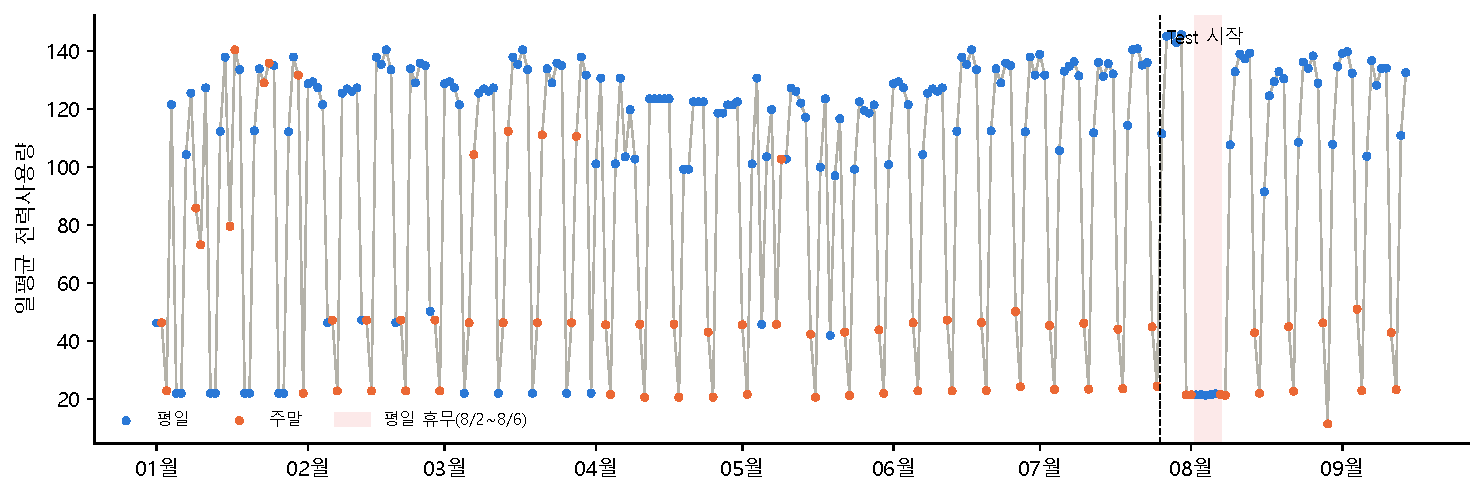
\includegraphics[width=\textwidth]{fig01_daily_power.pdf}
\caption{일평균 전력사용량. 평일과 주말의 차이가 크며, 8월 2일$\sim$6일은 평일임에도 주말 수준으로 떨어진다.}
\end{figure}

\begin{figure}[H]
\centering
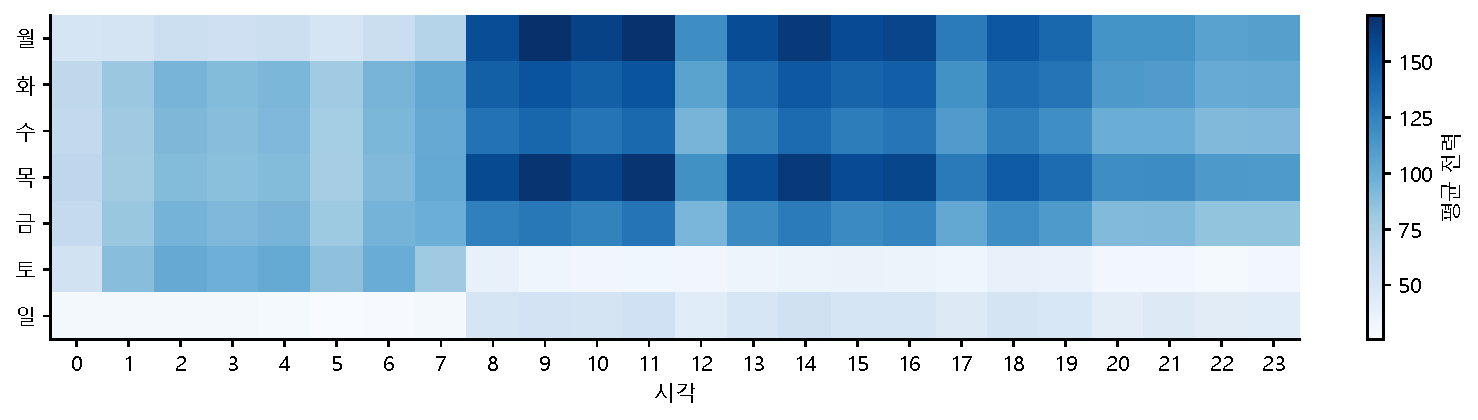
\includegraphics[width=\textwidth]{fig02_heatmap.pdf}
\caption{요일 $\times$ 시각별 평균 전력. 평일 오전 8$\sim$11시와 오후 13$\sim$16시에 부하가 집중되고, 12시(점심)에 일시적으로 감소한다.}
\end{figure}

\begin{itemize}
  \item 주말(토·일) 평균 전력은 41$\sim$51로 평일(103$\sim$123)의 절반 이하이다.
  \item 15분 전 전력과의 자기상관은 0.97로 매우 높아, 직전 값만으로도 상당한 예측력이 있다.
  \item 전력과의 상관이 가장 큰 변수는 생산량(0.51), 요일($-0.43$), 공장인원(0.29) 순이다.
\end{itemize}

\subsection{데이터 품질 점검}
\begin{warnbox}{발견된 데이터 문제}
\begin{itemize}[leftmargin=12pt]
  \item \textbf{생산 기록 누락:} 7월 13일과 15일은 생산량·공장인원이 하루 종일 0인데 일평균 전력은 약 136으로 평소 가동일 수준이다. 보조 파일 \code{okm\_augumented\_2021.csv}에서도 같은 두 날짜의 \code{시간} 값이 70$\sim$188로 깨져 있어 기록 오류로 판단하였다. 개선 모델에서는 해당일 생산량·공장인원을 결측으로 처리하였다.
  \item \textbf{생산량 0 $\neq$ 휴무:} 공휴일(2/11, 3/1)과 일부 일요일도 생산량은 0이지만 전력은 100 이상이다. 따라서 생산량만으로 휴무 여부를 판단할 수 없다.
  \item \textbf{평일 휴무:} 8월 2일$\sim$6일(월$\sim$금)은 전력이 약 21로 주말 수준이다. 여름휴가로 추정되며 Test 구간에 포함되어 있다.
\end{itemize}
\end{warnbox}

% ===============================================================
\section{초기 모델 (Feature4 XGBoost)}
% ===============================================================
\subsection{설계}
\begin{itemize}
  \item \textbf{Baseline:} 누수 변수(\code{평균}, \code{이상구간여부})를 제외한 13개 변수로 학습한 XGBoost.
  \item \textbf{Feature4:} Baseline 변수에 4개 파생변수를 추가하였다.
    \begin{itemize}
      \item \code{lag\_1\_power}: 15분 전 전력, \code{lag\_4\_power}: 1시간 전 전력
      \item \code{production\_change}: 직전 대비 생산량 변화
      \item \code{operation\_state}: 생산 전환 상태(비생산지속 / 생산시작 / 생산종료전환 / 생산지속)
    \end{itemize}
  \item \textbf{하이퍼파라미터:} \code{n\_estimators=500}, \code{learning\_rate=0.03}, \code{max\_depth=6},\newline \code{subsample=0.8}, \code{colsample\_bytree=0.8}.
  \item \textbf{검증:} 시간순 8:2 분할(Test: 2021-07-25 $\sim$ 09-14, 4,934행). TimeSeriesSplit 5-fold로 안정성을 확인하였다.
  \item \textbf{비교 기준:} Persistence, 즉 $\hat{P}_t = P_{t-1}$ (직전 값 그대로 사용).
\end{itemize}

\subsection{결과}
\begin{figure}[H]
\centering
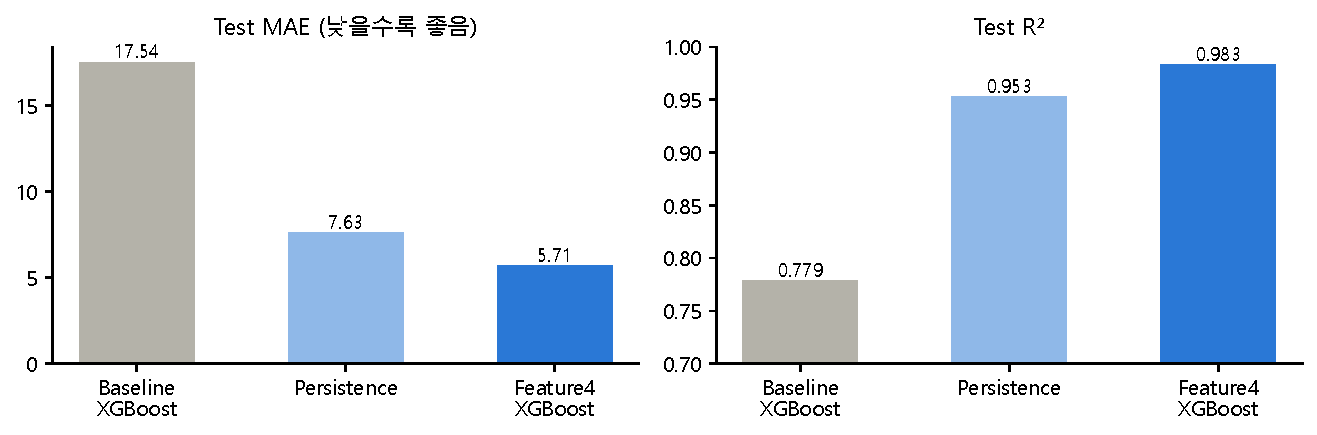
\includegraphics[width=0.85\textwidth]{fig05_original_comparison.pdf}
\caption{초기 모델 Test 성능 (원본 노트북 실행 결과)}
\end{figure}

\begin{table}[H]
\centering\small
\begin{tabular}{lrrrr}
\toprule
모델 & MAE & RMSE & $R^2$ & Train$-$Test $R^2$ 차이 \\
\midrule
Baseline XGBoost & 17.54 & 29.17 & 0.779 & 0.189 \\
Persistence & 7.63 & 13.50 & 0.953 & -- \\
Feature4 XGBoost & \textbf{5.71} & \textbf{8.20} & \textbf{0.983} & 0.006 \\
\bottomrule
\end{tabular}
\caption{초기 모델 성능 비교}
\end{table}

TimeSeriesSplit 5-fold 평균은 Feature4 $R^2=0.973$(표준편차 0.009), Persistence $R^2=0.941$로, 단일 분할 결과와 같은 경향을 보였다.

% ===============================================================
\section{초기 모델의 한계 진단}
% ===============================================================
\subsection{한계 1: 개선의 대부분은 lag 정보 자체에서 나온다}
Baseline에서 Feature4로 MAE가 17.5에서 5.7로 줄었지만, 학습 없이 직전 값을 베끼는 Persistence가 이미 7.6을 달성한다. 개선분 11.8 중 9.9는 ``15분 전 전력''이라는 정보 자체의 기여이고, 모델이 추가로 기여한 몫은 1.9이다. SHAP 분석에서도 \code{lag\_1\_power}의 평균 $|$SHAP$|$이 45.1로, 2위 \code{lag\_4\_power}(3.8)의 10배 이상이다.

이 정보는 15분 앞 예측에서만 쓸 수 있다. 그림~\ref{fig:decay}처럼 예측 구간이 길어지면 과거 값의 설명력은 급격히 떨어진다. 생산일정 조정에 필요한 몇 시간$\sim$하루 앞 예측에서는 초기 모델 구조를 그대로 쓸 수 없다.

\begin{figure}[H]
\centering
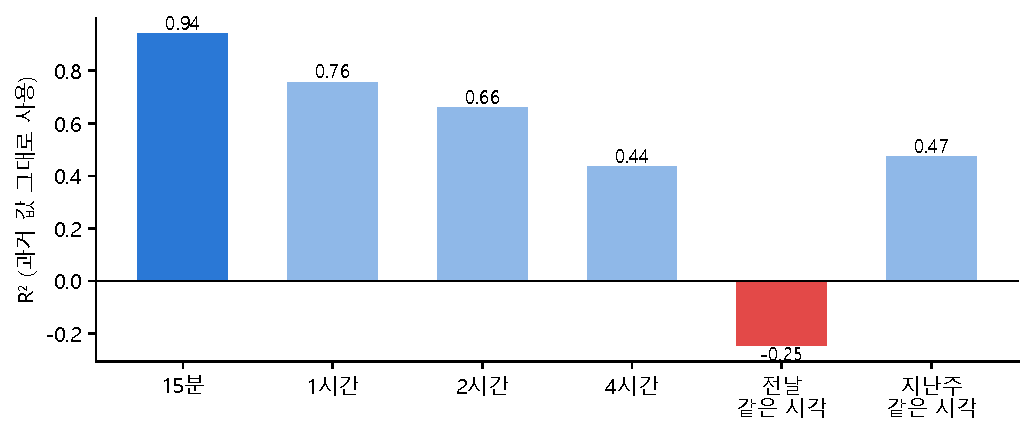
\includegraphics[width=0.7\textwidth]{fig04_persistence_decay.pdf}
\caption{예측 구간별 ``과거 값 그대로 쓰기''의 $R^2$ (전체 데이터). 전날 같은 시각 값은 주말·평일 전환 때문에 음수가 된다.}
\label{fig:decay}
\end{figure}

\subsection{한계 2: 시간 내 미래 정보 사용}
\begin{figure}[H]
\centering
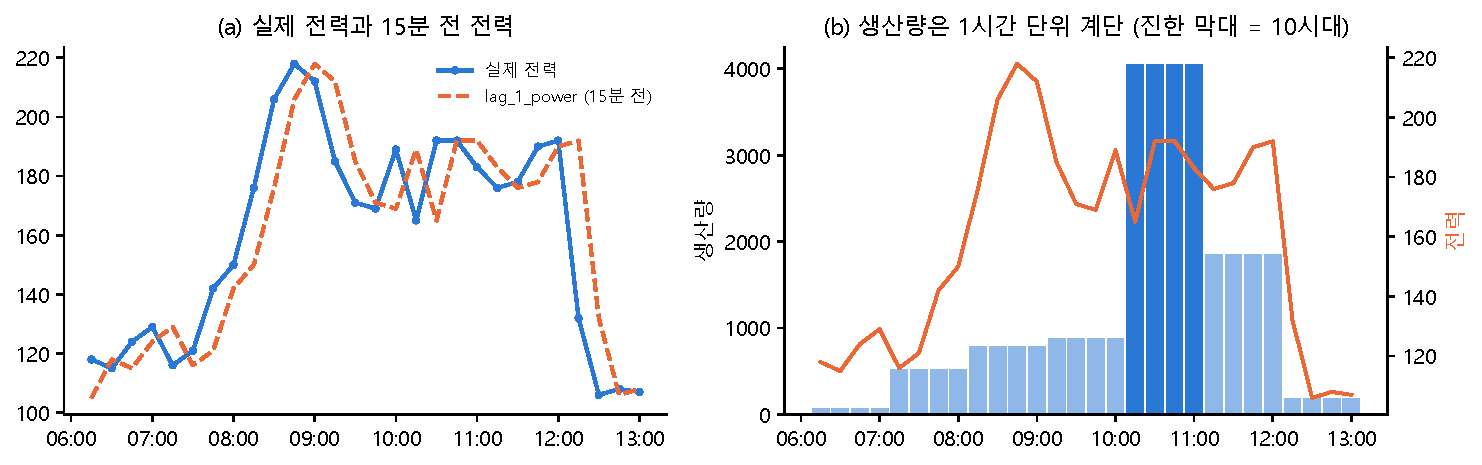
\includegraphics[width=\textwidth]{fig03_lag_and_leak.pdf}
\caption{2021-08-11 오전. (a) \code{lag\_1\_power}는 실제 전력을 한 칸 늦게 따라간다. (b) 생산량은 1시간 단위 실적이라 10:15 행에 이미 10시대 전체 생산량(4,050)이 들어 있다.}
\end{figure}

생산량은 1시간이 끝나야 확정되는 실적인데, 모델은 해당 시간의 첫 15분 행부터 이 값을 입력으로 받는다. 따라서 \code{production\_change}는 매시 15분 행에서만 0이 아니다. 기온 등 기상 변수도 같은 시각의 실제 관측값이다. 즉 초기 모델은 ``그 시각의 생산 실적과 날씨를 안다면''이라는 조건부 예측이다.

\subsection{한계 3: 피크 과소예측}
\begin{figure}[H]
\centering
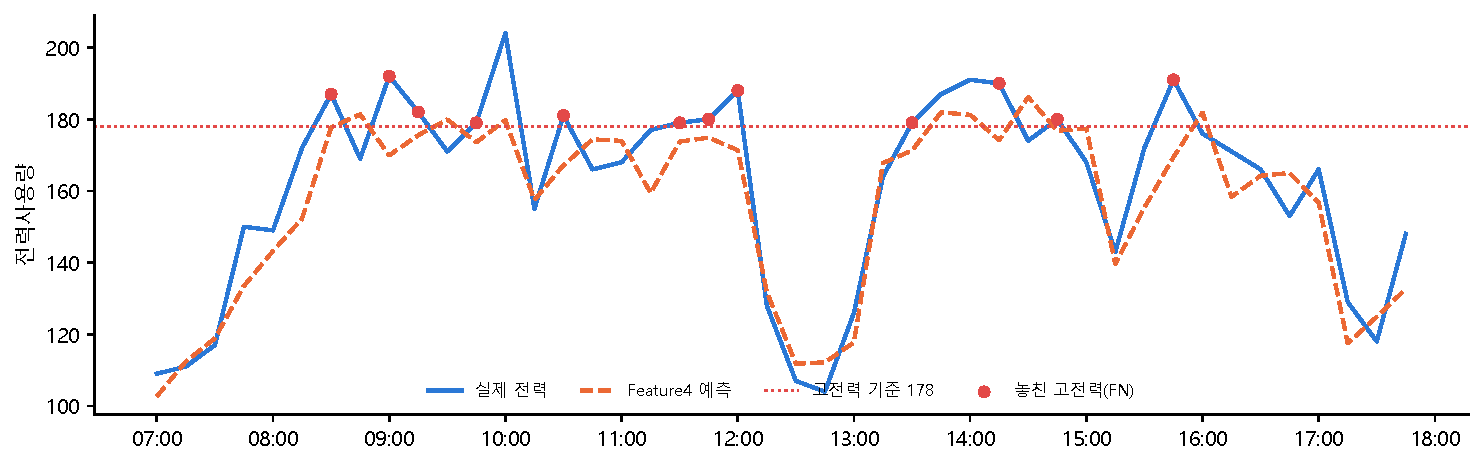
\includegraphics[width=\textwidth]{fig06_peak_underprediction.pdf}
\caption{2021-09-10 실제 전력과 Feature4 예측. 봉우리마다 예측이 실제보다 낮다.}
\end{figure}

\begin{table}[H]
\centering\small
\begin{tabular}{lrrrr}
\toprule
실제 전력 구간 & 건수 & 실제 평균 & 예측 평균 & 차이 \\
\midrule
100 $\sim$ 150 & 1,360 & 118.0 & 117.8 & $-0.2$ \\
150 $\sim$ 178 & 690 & 165.1 & 165.7 & $+0.6$ \\
178 $\sim$ 200 & 416 & 186.3 & 179.2 & $\mathbf{-7.1}$ \\
200 이상 & 65 & 204.7 & 192.0 & $\mathbf{-12.7}$ \\
\bottomrule
\end{tabular}
\caption{실제 전력 구간별 평균 예측값 (Test)}
\end{table}

실제 고전력(178 이상) 시점의 85\%에서 예측이 실제보다 낮았다. 제곱오차 목적함수는 불확실한 조건에서 예측을 평균 쪽으로 끌어당기기 때문에, 드문 피크일수록 낮게 예측된다. 그 결과 고전력 경보의 Recall은 0.62에 그쳐 실제 고전력 481건 중 182건을 놓쳤다.

\subsection{한계 4: 평일 휴무 미반영}
\begin{figure}[H]
\centering
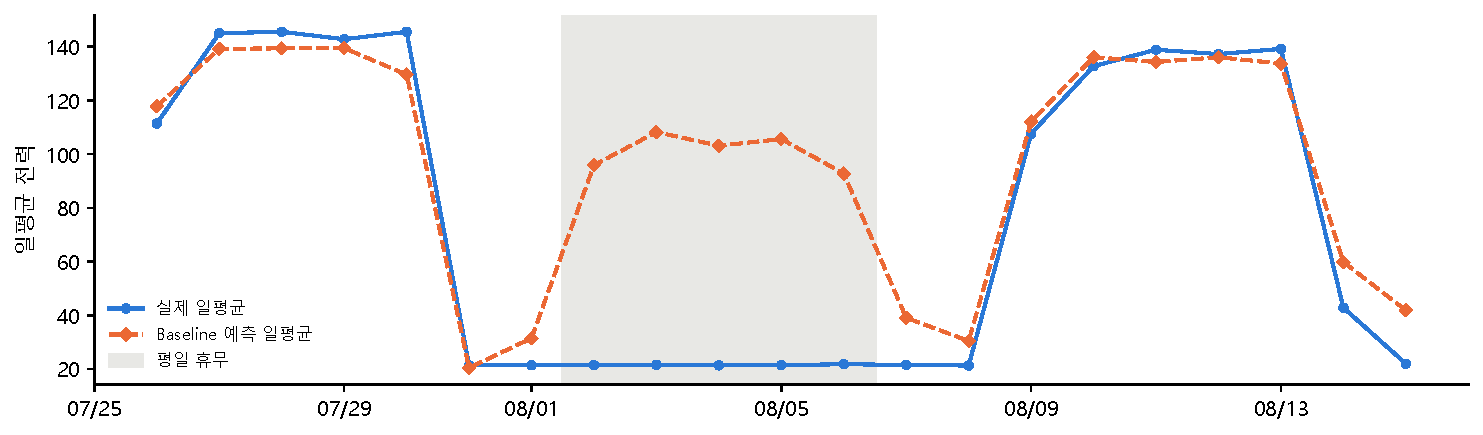
\includegraphics[width=\textwidth]{fig07_shutdown_baseline.pdf}
\caption{Test 구간 일평균 전력과 Baseline 예측. 8/2$\sim$8/6 평일 휴무를 평소 평일로 예측하였다.}
\end{figure}

휴무 주간에도 생산량·공장인원은 0으로 기록되어 있었다. 그러나 이 값은 평일 야간이나 점심시간에도 흔히 나타나므로, 모델은 이를 ``평일 중 잠시 생산이 없는 시간''으로 해석하였다. Baseline 대규모 오차 상위 5\%의 대부분이 이 주간에서 발생했다. 시간 단위 변수만으로는 ``하루 전체가 휴무''라는 정보를 표현할 수 없다.

% ===============================================================
\section{개선 모델 설계}
% ===============================================================
\subsection{예측 구간 분리}
15분($h=1$), 1시간($h=4$), 24시간($h=96$) 앞 예측 모델을 각각 학습하였다. 모든 전력 lag는 예측 구간 이상 떨어진 값만 사용하여, 예측 시점 $t-h$에 실제로 알 수 있는 정보만 입력된다.
\[
\text{lag} \in \{h,\; h+1,\; h+4,\; 96^{(h<96)},\; 672\},\qquad
\text{최근 1시간·24시간 평균} = \overline{P}_{[t-h-3,\,t-h]},\; \overline{P}_{[t-h-95,\,t-h]}
\]

\subsection{정보 가용성에 따른 두 시나리오}
\begin{table}[H]
\centering\small
\begin{tabular}{p{2.3cm}p{5.6cm}p{5.6cm}}
\toprule
 & 실적기반 & 계획기반 \\
\midrule
가정 & 예측 시점에 이미 끝난 정보만 사용 & 생산계획·기상예보를 미리 안다고 가정 \\
생산량 & 예측 시점까지 완료된 시간의 실적 & 대상 시각의 생산량(=계획) \\
공장인원 & 완료된 시간의 실적 & 대상 시각의 값(=계획) \\
기상 & 예측 시점의 관측값 & 대상 시각의 값(=예보) \\
의미 & 누수 없음. 지금 바로 운영 가능한 성능 & 생산계획 정보의 가치 \\
\bottomrule
\end{tabular}
\caption{시나리오 정의. 두 시나리오 모두 달력 변수와 전력 lag를 공통으로 사용한다.}
\end{table}

\subsection{휴무 반영과 데이터 보정}
\begin{itemize}
  \item \textbf{가동일 달력:} 일평균 전력이 30 미만인 날을 휴무일로 표시하였다(257일 중 49일, 평일 휴무 18일).
  \item \textbf{생산 기록 누락일 보정:} 7/13, 7/15의 생산량·공장인원을 결측 처리하였다.
\end{itemize}

\begin{warnbox}{가정 명시}
가동일 달력은 실제 전력으로 만든 대리 변수이다. 공장이 휴무 계획(여름휴가, 공휴일 등)을 사전에 알고 있다는 가정에 근거하며, 실제 적용 시에는 회사의 휴무 달력으로 대체해야 한다.
\end{warnbox}

\subsection{피크 대응}
\begin{itemize}
  \item \textbf{학습 가중치:} 고전력(Train 95\% 분위수 178 이상) 데이터에 가중치 3을 부여하였다.
  \item \textbf{경보 임계값 선택:} Train의 뒤쪽 20\%(2021-06-16 $\sim$ 07-25)를 검증 구간으로 두고, 검증 F1이 최대가 되는 예측 임계값을 선택하였다. Test는 임계값 선택에 사용하지 않았다.
\end{itemize}

% ===============================================================
\section{개선 결과}
% ===============================================================
Train은 lag 생성을 위해 앞쪽 800행을 제외한 18,938행이며, Test는 초기 모델과 동일한 4,934행이다. 비교를 위해 초기 Feature4도 같은 Train 행으로 다시 학습하였다.

\subsection{회귀 성능}
\begin{figure}[H]
\centering
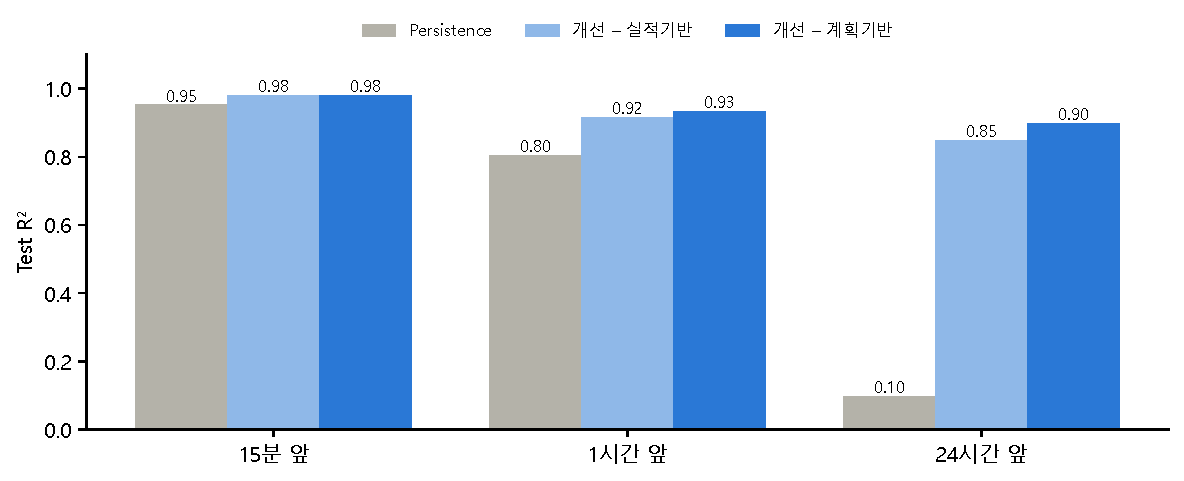
\includegraphics[width=0.8\textwidth]{fig09_improved_r2.pdf}
\caption{예측 구간별 Test $R^2$. 예측 구간이 길수록 Persistence 대비 개선 폭이 커진다.}
\end{figure}

\begin{table}[H]
\centering\small
\begin{tabular}{llrrrrr}
\toprule
예측 구간 & 모델 & MAE & $R^2$ & Pers. MAE & Pers. $R^2$ & MAE 개선 \\
\midrule
15분 앞 & 초기 Feature4 (재학습) & 6.23 & 0.980 & 7.63 & 0.953 & 1.39 \\
        & 개선 -- 실적기반 & 5.60 & 0.981 & 7.63 & 0.953 & 2.02 \\
        & 개선 -- 계획기반 & \textbf{5.50} & \textbf{0.981} & 7.63 & 0.953 & 2.13 \\
\midrule
1시간 앞 & 개선 -- 실적기반 & 11.51 & 0.916 & 16.16 & 0.804 & 4.65 \\
         & 개선 -- 계획기반 & \textbf{10.03} & \textbf{0.934} & 16.16 & 0.804 & 6.13 \\
\midrule
24시간 앞 & 개선 -- 실적기반 & 15.29 & 0.849 & 33.85 & 0.096 & 18.56 \\
          & 개선 -- 계획기반 & \textbf{12.51} & \textbf{0.898} & 33.85 & 0.096 & 21.34 \\
\bottomrule
\end{tabular}
\caption{개선 모델 회귀 성능 (Test)}
\end{table}

\begin{itemize}
  \item 15분 앞에서는 실적기반과 계획기반의 차이가 작다(MAE 5.60 vs 5.50). 초기 모델의 시간 내 미래 정보 사용은 단기 예측 성능을 크게 부풀리지 않았다.
  \item 24시간 앞에서는 생산계획을 알면 MAE가 15.3에서 12.5로 줄어든다. 생산계획 정보의 가치를 보여준다.
\end{itemize}

\subsection{개선 요소별 기여 (24시간 앞, 계획기반)}
\begin{table}[H]
\centering\small
\begin{tabular}{lrrr}
\toprule
구성 & MAE & $R^2$ & 경보 F1 (검증선택) \\
\midrule
전체 (가동일 달력 + 고전력 가중치) & 12.51 & 0.898 & 0.576 \\
가동일 달력 제외 & 20.06 & 0.728 & 0.569 \\
고전력 가중치 제외 & 12.54 & 0.900 & 0.576 \\
\bottomrule
\end{tabular}
\caption{Ablation. 가동일 달력의 효과가 가장 크고, 고전력 가중치의 효과는 미미하다.}
\end{table}

\begin{figure}[H]
\centering
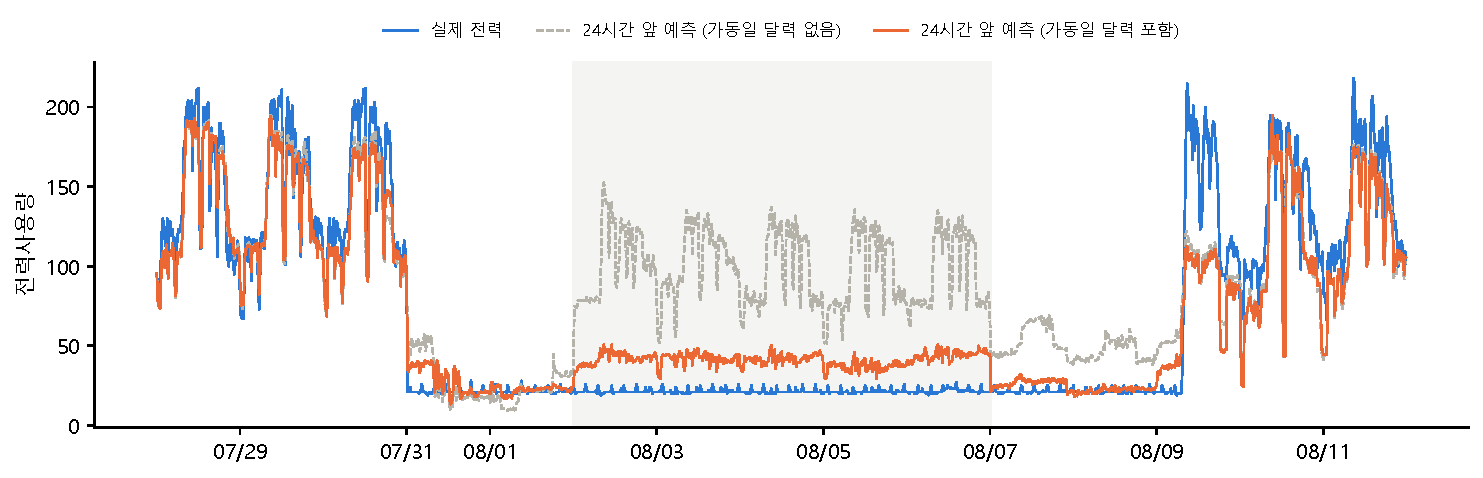
\includegraphics[width=\textwidth]{fig10_calendar_effect.pdf}
\caption{24시간 앞 예측의 휴무 주간 전후. 가동일 달력이 없으면 휴무 주간을 평일 수준으로 예측한다.}
\end{figure}

\begin{figure}[H]
\centering
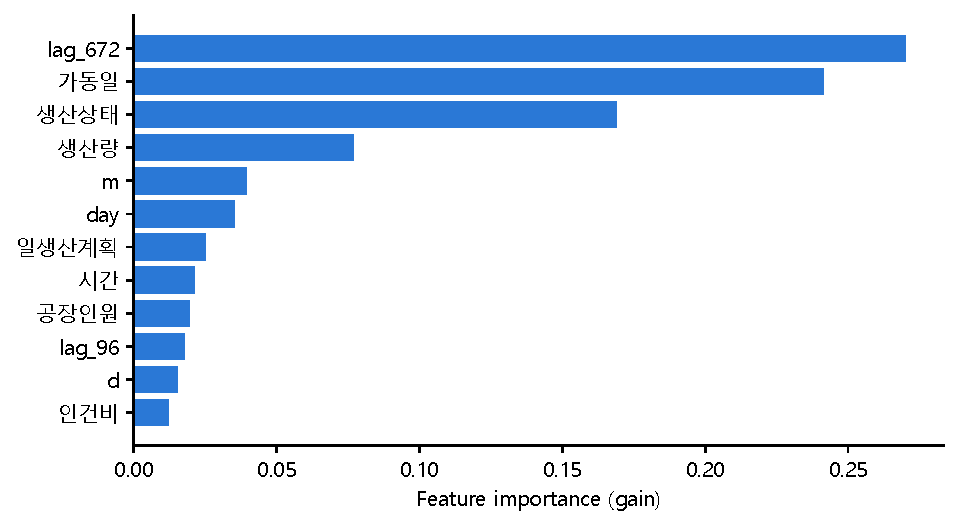
\includegraphics[width=0.62\textwidth]{fig12_importance_24h.pdf}
\caption{24시간 앞(계획기반) 모델 변수 중요도 상위 12. 1주 전 같은 시각 전력, 가동일, 생산상태, 생산량 순이다.}
\end{figure}

\subsection{고전력 경보 성능}
\begin{figure}[H]
\centering
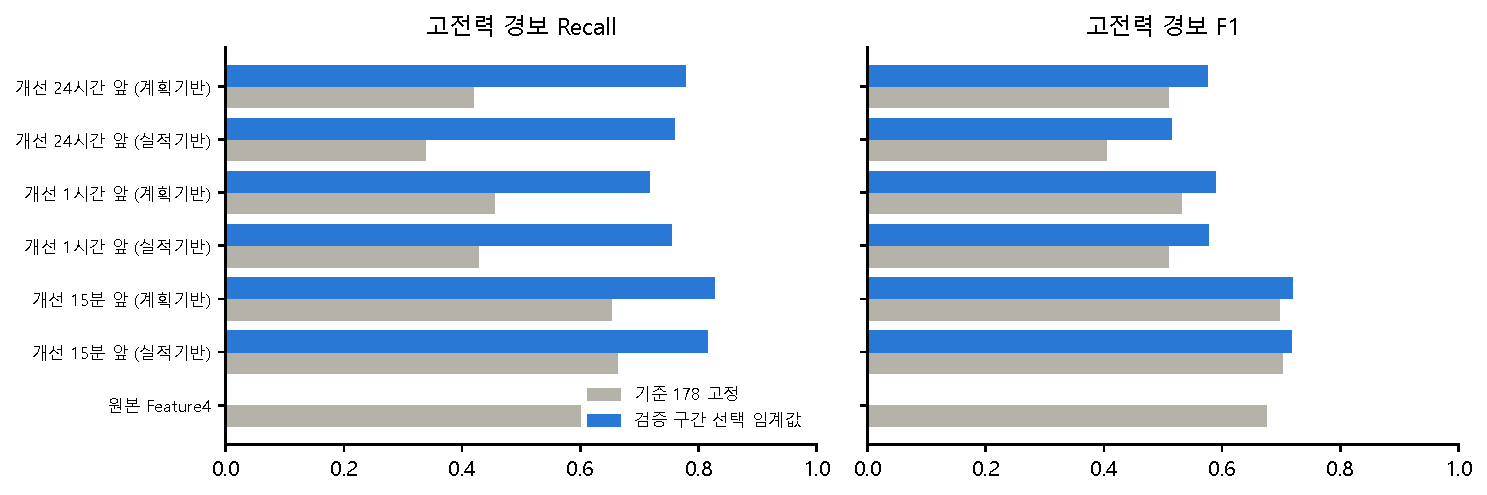
\includegraphics[width=\textwidth]{fig11_alarm.pdf}
\caption{고전력 경보 Recall과 F1. 정답은 실제 전력 $\ge 178$이다.}
\end{figure}

\begin{table}[H]
\centering\small
\begin{tabular}{lrrrrrrr}
\toprule
 & \multicolumn{3}{c}{기준 178 고정} & & \multicolumn{3}{c}{검증 선택 임계값} \\
\cmidrule{2-4}\cmidrule{6-8}
모델 & Precision & Recall & F1 & 임계값 & Precision & Recall & F1 \\
\midrule
초기 Feature4 (재학습) & 0.773 & 0.601 & 0.676 & -- & -- & -- & -- \\
15분 앞 실적기반 & 0.745 & 0.663 & 0.702 & 173 & 0.642 & 0.815 & 0.718 \\
15분 앞 계획기반 & 0.749 & 0.653 & 0.698 & 172 & 0.637 & 0.827 & \textbf{0.720} \\
1시간 앞 실적기반 & 0.628 & 0.428 & 0.509 & 165 & 0.467 & 0.755 & 0.577 \\
1시간 앞 계획기반 & 0.638 & 0.455 & 0.532 & 169 & 0.501 & 0.717 & 0.590 \\
24시간 앞 실적기반 & 0.503 & 0.339 & 0.405 & 154 & 0.390 & 0.759 & 0.515 \\
24시간 앞 계획기반 & 0.645 & 0.420 & 0.509 & 164 & 0.457 & 0.778 & 0.576 \\
\bottomrule
\end{tabular}
\caption{고전력 경보 성능 (Test)}
\end{table}

임계값을 낮추면 Recall은 크게 오르고 Precision은 내려간다. 피크를 놓치는 비용(최대수요전력 상승에 따른 기본요금 증가)이 불필요한 경보의 비용보다 크다는 판단에 따라 Recall 쪽을 선택하였다. 실제 운영에서는 두 오류의 비용을 정한 뒤 임계값을 다시 선택해야 한다.

% ===============================================================
\section{예측오차 및 최대피크 발생 조건 분석}
% ===============================================================
본 장의 수치는 초기 Feature4 모델의 Test 구간 결과이다.

\subsection{예측오차가 큰 생산조건}
절대오차 상위 5\%(17.2 이상, 247건)를 대규모 오차로 정의하였다.

\begin{table}[H]
\centering\small
\begin{tabular}{llrrr}
\toprule
구분 & 조건 & 건수 & 평균 절대오차 & 대규모 오차율 \\
\midrule
생산량 구간 & 생산량 = 0 & 2,062 & 3.44 & 2.8\% \\
 & 생산량 1,238 초과 & 716 & 8.56 & \textbf{9.8\%} \\
생산량 변화 & 증가 & 404 & 8.30 & \textbf{9.2\%} \\
 & 감소 & 346 & 7.82 & 7.5\% \\
 & 변화 없음 & 4,184 & 5.28 & 4.4\% \\
생산 상태 & 생산시작 & 34 & 8.57 & 8.8\% \\
 & 생산지속 & 2,838 & 7.31 & 6.6\% \\
 & 비생산지속 & 2,029 & 3.38 & 2.8\% \\
공장인원 & 인원 $>$ 0 & 2,940 & 7.56 & \textbf{7.6\%} \\
 & 인원 = 0 & 1,994 & 2.97 & 1.2\% \\
\bottomrule
\end{tabular}
\caption{조건별 대규모 오차율 (전체 평균 5\%)}
\end{table}

\begin{itemize}
  \item 오차는 \textbf{생산 중, 특히 고생산량 구간과 생산량이 바뀌는 시점}에 집중된다. 비생산 구간의 오차는 작다.
  \item 대규모 오차 247건 중 과소예측은 121건(실제 평균 165.9, 예측 143.5), 과대예측은 126건(실제 83.3, 예측 105.3)이다. 고부하는 낮게, 부하 감소는 늦게 따라가는 경향이 있다.
  \item 고전력 경보의 FN율(실제 고전력 중 놓친 비율)은 18시 81\%, 16시 61\%, 15시 53\%로 \textbf{오후 부하 감소 직전}에 높았다. FP율은 9시(12.6\%), 14시(11.1\%), 11시(10.8\%)에 높았다.
\end{itemize}

\subsection{최대전력 피크 발생 조건}
월별 최대피크는 각 월의 15분 관측값 중 최댓값으로 정의하였다(9건, 동률 없음). 표본이 적으므로 각 월 상위 5\%(1,298건)를 고전력 위험구간으로 정의하여 보조 분석하였다.

\begin{figure}[H]
\centering
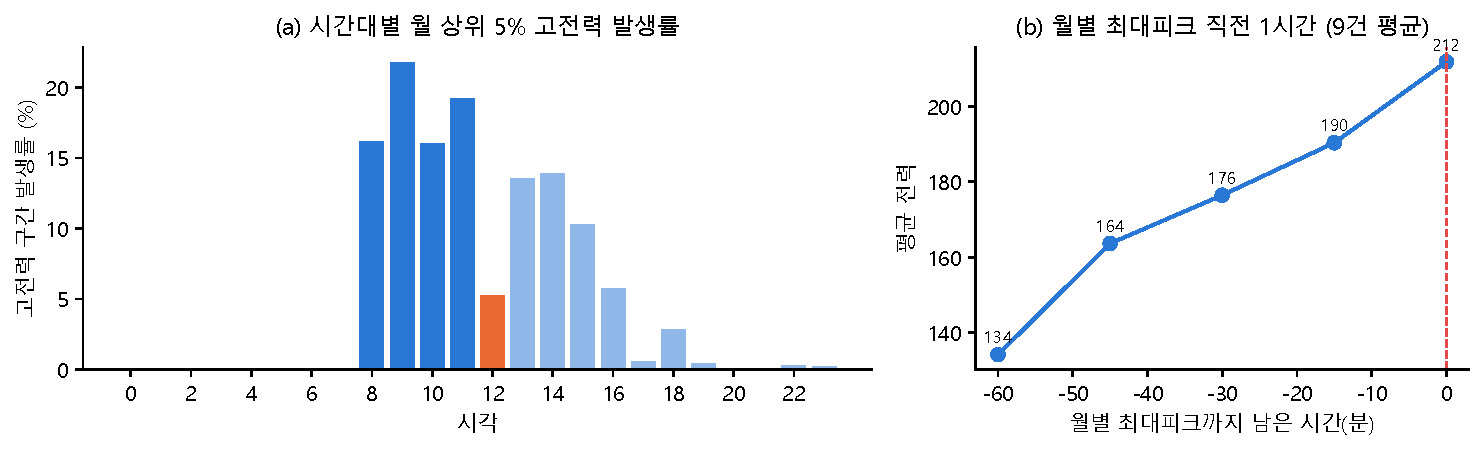
\includegraphics[width=\textwidth]{fig08_peak_conditions.pdf}
\caption{(a) 시간대별 고전력 위험구간 발생률. 8$\sim$11시에 집중되고 12시에 급감하며, 17시 이후에는 3\% 미만이다. (b) 월별 최대피크 직전 1시간의 평균 전력.}
\end{figure}

\begin{table}[H]
\centering\small
\begin{tabular}{lp{5.2cm}p{6.2cm}}
\toprule
조건 & 월별 최대피크 (9건) & 고전력 위험구간 (월 상위 5\%) \\
\midrule
시간대 & 9건 모두 08:30$\sim$11:30 & 9시 발생률 21.8\% (전체 대비 4.1배) \\
생산 상태 & 9건 모두 생산지속 & 생산지속이 90.1\% 차지 (1.6배) \\
생산량 & 중앙값 783 (전체 중앙값 45) & 498$\sim$1,175 구간이 41.9\% 차지 (3.0배) \\
생산량 변화 & 9건 모두 변화 없음 & 변화 없음 87.6\% (1.03배) \\
공장인원 & 9건 모두 인원 $>$ 0 & 인원 $>$ 0이 90.4\% 차지 (1.6배) \\
\bottomrule
\end{tabular}
\caption{피크 발생 조건. 괄호는 전체 데이터 비율 대비 집중도이다.}
\end{table}

\begin{keybox}{피크 발생 메커니즘 해석}
최대피크는 생산량이 급변하는 순간이 아니라, \textbf{아침 가동 후 중간 이상 생산량으로 생산이 지속되는 오전 시간대}에 발생한다. 피크 직전 1시간 평균 전력은 134 $\rightarrow$ 164 $\rightarrow$ 176 $\rightarrow$ 190 $\rightarrow$ 212로 15분마다 계단식으로 상승한다. 오전에 설비가 순차적으로 추가 가동되며 부하가 누적되는 패턴으로 해석된다. 단, 설비별 데이터가 없어 이 해석은 연관성에 근거하며 인과관계를 입증하지 않는다.
\end{keybox}

% ===============================================================
\section{피크전력 저감방안}
% ===============================================================
제7장의 분석을 근거로 다음 방안을 제안한다.

\begin{enumerate}[label=\textbf{방안 \arabic*.},leftmargin=*]
  \item \textbf{아침 설비 가동 순차화.} 피크 직전 1시간 동안 전력이 78 상승한다. 8$\sim$9시에 설비를 동시에 가동하지 말고 15$\sim$30분 간격으로 순차 가동하여 상승 기울기를 완만하게 만든다.
  \item \textbf{오전 고부하 생산의 시간대 이동.} 고전력 발생률은 9시 21.8\%, 11시 19.3\%인 반면 12시는 5.3\%, 17시 이후는 3\% 미만이다. 생산량 498$\sim$1,175 구간의 오전 작업 일부를 점심 직후나 17시 이후로 옮긴다. 야간으로 옮길 경우 인건비 계수(1.5)를 함께 고려해야 한다.
  \item \textbf{예측 기반 2단계 운영.}
    \begin{itemize}
      \item 전날: 24시간 앞 계획기반 모델로 다음 날 시간대별 전력을 예측하고, 고전력이 예상되는 시간대의 생산계획을 조정한다.
      \item 당일: 15분 앞 모델의 경보(검증 선택 임계값, Recall 0.82)로 피크 직전에 비필수 부하를 일시 차단한다.
    \end{itemize}
  \item \textbf{오후 부하 감소 구간의 경보 보완.} 15$\sim$18시는 FN율이 높으므로 이 시간대에는 경보 임계값을 별도로 낮게 설정하는 것을 검토한다.
\end{enumerate}

\begin{warnbox}{정량 효과 검증은 향후 과제}
위 방안의 피크 저감량과 비용 절감액은 아직 정량화하지 않았다. 24시간 앞 계획기반 모델은 생산계획을 입력으로 받으므로, 생산량을 다른 시간대로 옮긴 시나리오를 입력해 월별 최대전력 변화를 시뮬레이션할 수 있다. 줄어든 최대전력에 기본요금 단가를 곱해 절감액도 추정할 수 있다.
\end{warnbox}

% ===============================================================
\section{한계 및 향후 과제}
% ===============================================================
\begin{itemize}
  \item \textbf{가동일 달력 가정:} 실제 전력으로 만든 대리 변수이므로, 회사의 휴무 달력으로 대체한 뒤 재평가해야 한다. 이 변수가 없으면 24시간 앞 $R^2$는 0.73이다.
  \item \textbf{Test 독립성:} 개선 방향을 정하는 과정에서 Test 결과를 참고한 실험이 있었다. 최종 설계는 고정 규칙을 사용했으나, 완전히 독립된 평가를 위해 별도 기간(예: 2021년 10월 이후) 데이터로 재검증이 필요하다.
  \item \textbf{계획 정보:} 계획기반 시나리오는 실적을 계획으로 간주한 것이다. 실제 생산계획과 실적의 차이가 있으면 성능이 낮아질 수 있다.
  \item \textbf{데이터 기간:} 1$\sim$9월 데이터로 겨울철 난방 부하나 연말 패턴은 학습되지 않았다.
  \item \textbf{설비 단위 정보 부재:} 설비별 전력이나 가동 기록이 있으면 동시 가동의 영향을 직접 분석할 수 있다.
\end{itemize}

% ===============================================================
\appendix
\section{재현 방법}
% ===============================================================
\begin{table}[H]
\centering\small
\begin{tabular}{p{5.2cm}p{9cm}}
\toprule
파일 & 내용 \\
\midrule
\code{KAMP\_modeling\_3\_7.py} & 초기 모델 전체 분석 (Baseline, Feature4, 오차·피크·경보·SHAP 분석) \\
\code{KAMP\_modeling\_improved.py} & 개선 모델 (예측 구간 $\times$ 시나리오, Ablation, 그림) \\
\code{report/make\_figures.py} & 보고서 그림 생성 \\
\code{outputs/} & 예측 결과 및 분석표 CSV \\
\bottomrule
\end{tabular}
\end{table}

실행 환경: Python 3, pandas 3.0, scikit-learn 1.9, xgboost 3.4.\\
각 스크립트를 데이터 파일 \code{Power15MinClean\_NoDatetime.csv}와 같은 폴더에 두고 Spyder에서 실행한다.\\
초기 모델 수치는 원본 노트북(Colab) 결과이며, 패키지 버전에 따라 소수점 셋째 자리에서 차이가 날 수 있다.

\end{document}
